\documentclass[./thesis.tex]{subfiles}

 
\begin{document}

\label{chap:exp_dressing}

While CI methods are common ways to account for electron correlation, they suffer a severe size consistency problem.


The logics of the electronic Many-Body problem has been clarified a long time
ago in the situations where  the  wave  function  may  be  generated  from  a
single  determinant  (or  single  reference).  Perturbative  developments,
translated  in  terms  of  diagrams,  led  to  the  formulation  of  the
fundamental  linked  cluster  theorem,\cite{Goldstone}  and  clarified  the  defects  of
truncated  Configuration Interaction  methods.  The  conditions  for  a  good
scaling  of  the  correlation  energy  and  for  the  strict separability  into
closed  shell  fragments  were  established.

By  strict  separability  (which
is  less ambiguous than the terms size-extensivity and size consistency) we
mean that at the non-interacting limit of an $A\cdots B$ problem the energies are
additive, $E_{A\cdots B} = E_A+E_B$, and that the amplitudes associated with the single
and  double excitation operators  are  the  same  as  those  obtained  for  the  isolated  $A$
and  $B$  problems.

Why this is not the case in CI methods can be easily understood as the absence of some excitations simulatenously on all subsystems.

Considering a supersystem $C$ made of two non-interacting subsystems $A$ and $B$, and write its CID wavefunction (Hartree-Fock determinant and all its double excitations).

\begin{equation}
\Psi^C = \Psi_{HF}^C + \Psi_{D}^C
\end{equation}

with $\Psi_{HF}^C$ the Hartree-Fock determinant for system $C$, and $\Psi_{D}^C$ the sum of all double excitation with respect to $\Psi_{HF}^C$.

If we now write $\Psi^{A+B}$ the product of the two separate CID wavefunctions of $A$ and $B$


\begin{align}
\Psi^{A+B} = & \Psi^A  \Psi^B \\
 = & \Psi_{HF}^A\Psi_{HF}^B  + \Psi_{HF}^A\Psi_{D}^B + \Psi_{D}^A\Psi_{HF}^B + \Psi_{D}^A \Psi_{D}^B \\
 = & \Psi^C_{HF} + \Psi^C_D + \Psi_{D}^A \Psi_{D}^B
\end{align}

As can be seen, $C$ isn't described as the product of $A+B$ as it should, since simultaneous double excitations on $A$ and $B$ cannot be accounted for

\begin{equation}
\Psi^{A+B} - \Psi^C  = \Psi_{D}^A \Psi_{D}^B
\end{equation}

Some methods aim at partially or fully correct this size-consistency error by eliminating the unlinked effects of the CISD. The so-called \emph{Davidson corrections}, that are essentially correction to the energy\cite{Langhoff_1974}. \alert{citation a verif}, and the so-called \emph{Coulpled Electron Pair Approximations (CEPA)} that correct the CI equations\cite{Kelly_1963,Kelly_1964,Meyer_1971,Meyer_1973,Meyer_1974,Ahlrichs_1975}. Many different variations have been proposed, for a review see \cite{Koch_1981}.






\begin{algorithm}
\KwData{$\kalpha$ the considered exernal determinant}
\KwData{$D_i$ the list of $N$ internal determinants connected to $\kalpha$}
\KwResult{finds all diamonds in $\mathcal{O}(N_{ref} \times N)$} 

\ForAll{$\kI$ with $EXC(\kI, \kalpha) \leq 4$}{

$\delta \gets -(I + \alpha)$ \;
$i \gets 1$ \;
$j \gets 1$ \;
\While{$j \leq N \wedge i \leq N$}{
	\uIf{$D_j - D_i > \delta$}{
		increment $i$ \;
	}
	\uElseIf{$D_j - D_i < \delta$}{
		increment $j$ \;
	}
	\Else
	{
		\tcc{$\hat T_{I \rightarrow D_j}$ is $D_j-I$}
		\tcc{$D_i + (D_j-I) = \alpha$}
		
		
		
		%\tcc{\alert{check diamond}}
		%\If{$(I \oplus D_i \wedge I = D_j \oplus \alpha \wedge D_j) \wedge (I \oplus D_i \wedge D_i = D_j \oplus \alpha \wedge \alpha)$}{
		%\If{$\hat T_{I \rightarrow D_i} = \hat T_{D_j \rightarrow \alpha}$}{
		
		\tcc{\alert{check if addition applies correct excitaion}}
		\tcc{impossible exciation results in an abnormal number of modified spinorbitals}	
		\If{$||D_j \oplus I|| = ||D_i \oplus \alpha||$}{
			diamond found \;
		}
		increment $i$ and $j$ \;
	}
}
}
\end{algorithm}

Applying an impossible excitation by addition, will usually lead to an abnormal result with a wrong number of ``electrons''. But in some cases, it may lead to an existing determinant. 



This algorithm works when bitstrings are considered binary integers of arbitrary size. However, no assumption is made about the operators involved in the diamond, they can be any combination of creations and anihilations. Therefore, for simplification purpose, it is possible to consider all 64-bit integers independently, each one carrying a subset of the operators involved in the excitation.

Essentially, adding and substracting can be done integer-wise, without the added complexity of carry and overflow.
Because integers of lower $\Nint$ vary more, they should be given more weight when comparing, as this will allow to shorcut the loop over $\Nint$ faster.

\section{Computing $c_\alpha$}
Whether the matrix dressing algorithm performs a shifted-Bk, an MR-CCSD or some other method, depends on the external space, i.e. the $c_\alpha$ coefficients. Our goal is to set up a framework in which stochastic matrix dressing can be done efficiently in an external space only defined by $Z(\alpha)$ a function that takes a determinant and returns the $c_\alpha$ it should be associated with.
Looking at the expression of $c_\alpha$ for shifted-Bk, it looks like the computation required is the exact same as the one performed by our CIPSI

\begin{equation}
c_\alpha = \frac{\Hij{\alpha}{\Psi}}{\Delta E}
\end{equation}


But the expression of $c_\alpha$ for shifted-Bk has a particularity that lifts a constraint compared to the general case: as can be seen, while for any $\kalpha$ we need to find all internal determinants it connects to, we do not need to know them \emph{at the same time}. This is not generally the case, as can be told by the expression of $c_\alpha$ for MRCC.

Thus, matrix dressing generally requires knowledge of all internal determiants a particular $\kalpha$ connects to, before $c_\alpha$ - and thus the associated increment to $\kappa$ - can be computed. For efficiency, as well as simplicity, this list must absolutely be computed upstream the call to $Z(\alpha)$, therefore making it $Z^\star(\alpha, \Psi_{c})$ with $\Psi_{c}$ the variational wavefunction stripped of all determinants that do not connect to $\kalpha$ (thus not normalized). 

This is a lot like the former implementation of CIPSI : considering one $\kalpha$ at a time, enumerate its connections to selectors. The new, more efficient algorithm, however, considers a batch of up to ${N_{virt}}^2$ rather than a single one. The solution in conceptually simple. Neglecting connections to determinants that are not selectors :
\begin{enumerate}
\item
Iterate over all $G_{pq}$ batches in the same way as in the CIPSI algorithm, building the $B_{rs}$ tag matrix
\item
create ${(2N_{orb})}^2$ determinant sets $\mathcal{C}_{rs}$ each associated with $\Gpqrs$
\item
when a connection between a selector $\ket S$ and $\kalpha = \ket {G_{pq}^{rs}}$ is found, add $\ket S$ to $\mathcal{C}_{rs}$ (instead of incrementing $P(G_{pq})$).
\item
for each untagged $\kalpha = \Gpqrs$ call $Z^\star(\alpha, \mathcal{C}_{rs})$
\end{enumerate}


\begin{figure}[h!]
	\begin{center}
		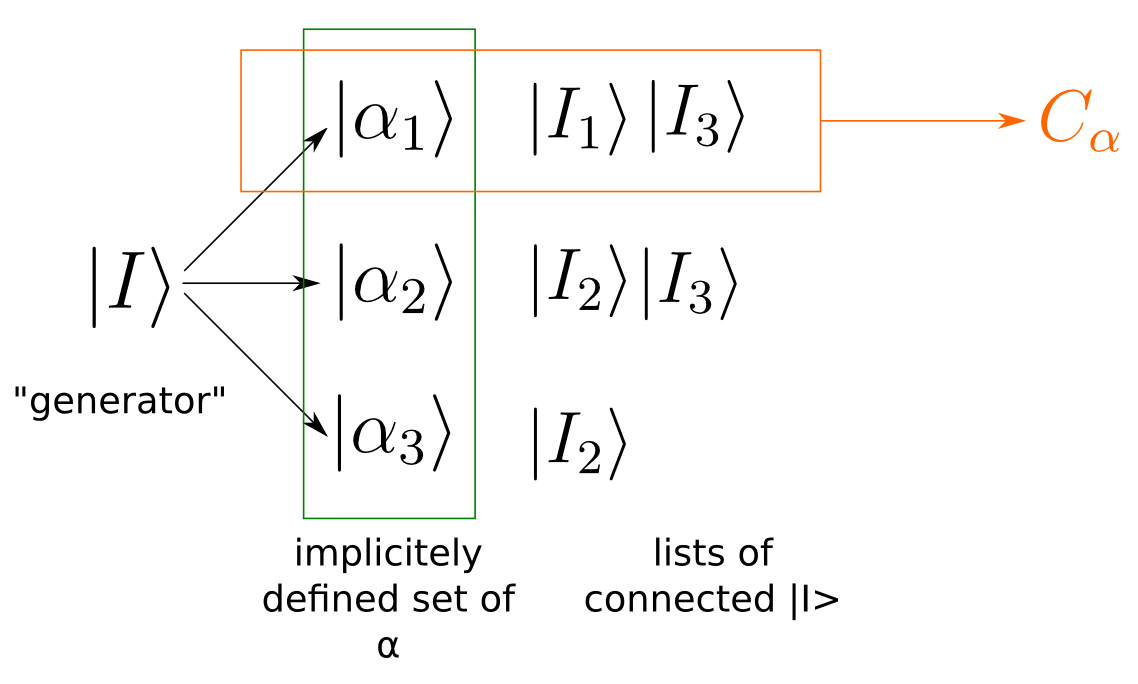
\includegraphics[width=0.7\columnwidth]{figures/matrix_dressing/buildlists}
		\caption{A REFAIRE NOTATION.............}
		\label{fig:buildlists}
	\end{center}
\end{figure}

When computation for batch $G_{pq}$ is completed, $\mathcal{C}_{rs}$ is the set of all selectors $\ket S$ connecting to $\kalpha$. As can be seen, this is pretty much the CIPSI algorithm, except we are building sets instead of incrementing scalars. This, of course, adds implementation complexity. The sizes of the $\mathcal{C}_{rs}$ sets aren't known in advance. Resizable arrays can be used. While they are not very practical to use in Fortran, they are not too hard to set up. 

More importantly, the storage space required may be concerningly high. Noticing that :
\begin{itemize}
\item
all $\Gpqrs$ in a batch are connected to each other
\item
there is ${N_{virt}}^2$ non-null $\Gpqrs$ in a batch
\end{itemize}
and considering
\begin{itemize}
\item
$G_{pq}$ the first batch (all generated $\kalpha$ are unique)
\item
half of $\Gpqrs$ are internal determinants
\end{itemize}

We have ${N_{virt}}^2 / 2$ unique $\kalpha$ in the batch each one connecting to at least ${N_{virt}}^2 / 2$ internal determinants, for a total storage space of at least ${N_{virt}}^4 / 4$.
This case isn't irrealistic, with $\ket {G_{pq}}$ the Hartree-Fock determinant with $(p,q)$ the HOMO spinorbitals.

Another issue is a high number of non-contiguous writes in memory, especially with those selectors that connect to all determinants of the batch ; they need to be added to ${N_{virt}}^2$ sets, which is ${N_{virt}}^2$ non-contiguous writes for a single selector.

We can solve the storage issue and mitigate the number of non-contiguous writes, by creating sets of $\kalpha$ that are subsets of several $\mathcal{C}_{rs}$.
Table \ref{tab:systematic_determination} indicates which $\kalpha = \ket {G_{pq}^{rs}}$ of the current batch a selector $\kS$ connects to. In some cases, there are ``wildcard'' indices $X$ and $Y$. Instead of looping over the possible values for those wildcards and adding $\kS$ to all the corresponding $\mathcal{C}_{rs}$ sets, we are going to give wildcard indices the special value $0$ and build intermediate sets $\tilde{\mathcal{C}}_{rs}$. For example, in the case where both $r$ and $s$ are wildcards, instead of adding $\kS$ to all $\mathcal{C}_{rs}$ sets, we will add it to a single set $\tilde{\mathcal{C}}_{00}$. When computation for the batch is completed, $\mathcal{C}_{rs}$ can be evaluated as

\begin{equation}
\mathcal{C}_{rs} \gets \tilde{\mathcal{C}}_{rs} \cup \tilde{\mathcal{C}}_{r0} \cup \tilde{\mathcal{C}}_{s0} \cup \tilde{\mathcal{C}}_{00}
\end{equation}

Care must be given that $\tilde{\mathcal{C}}_{r0}$ and $\tilde{\mathcal{C}}_{s0}$ may share common elements. Given its frequency, it is important that this computation be efficient. As is sometimes the case, efficiency implies $\mathcal{C}_{rs}$ are not computed individually, but become available inside a loop. An implementation is proposed as algorithm \ref{alg:compute_connected}, which tries to reuse shared $\tilde{\mathcal{C}}_{rs}$ as much as possible.


\newcommand{\interC}[1]{\tilde{\mathcal{C}}_{#1}}
\newcommand{\finC}[1]{\mathcal{C}_{#1}}

\begin{algorithm}
	\caption{Build $\mathcal{C}_{rs}$ from $\tilde{\mathcal{C}}_{rs}$}
	\label{alg:compute_connected}
	\tcc{This takes place after $\tilde{\mathcal{C}}_{rs}$ and $B_{rs}$ for a given batch have been fully computed}
		\KwData{$\tilde{\mathcal{C}}_{rs}$ the intermediate sets, $B_{rs}$ the tag matrix}
		%\KwResult{$Z^\star(\Gpqrs, \mathcal{C}_{rs})$ is called for all $\Gpqrs$ of $G_{pq}$ batch that are unique $\kalpha$}
		\KwResult{$\mathcal{C}_{rs}$ is computed for all $\Gpqrs$ of $G_{pq}$ batch that are unique $\kalpha$} 
		\tcc{$\interC{rs}$ and $\finC{rs}$ are considered arrays, the syntax $\finC{rs}[i\ldots j]$ is used to denote a segment of array}
		$T$ and array size $\Nsel$ initialized to TRUE \;
		$L$ an array of determinants size $\Nsel$ \;
        $i_1 = |\interC{00}|$ \;   
        $L[1 \ldots i_1] \gets \interC{00}[1 \ldots {i_1}]$ \;
        
		\tcc {$B_{r0} = FALSE$ if column entirely tagged}		
		\ForAll{$r ; B_{r0}$}{
		  $i_2 = i_1 + |\interC{r0}|$ \;
		  $L[i_1+1 \ldots i_2] \gets \interC{r0}$ \;
		  \For{$i=1,|\interC{r0}|$}{
		    $T[\interC{r0}[i]] \gets FALSE$
		  }
		  \ForAll{$s;B_{rs}=TRUE$}{
		    $i_3 = i_2$ \;
		    \For{$i=1,|\interC{s0}|$}{
		      \If{$T[\interC{s0}[i]]$}{
		        $i_3 \gets i_3+1$ \;
		        $L[i_3] \gets \interC{s0}[i]$ \;
		      }
		    }
		    
		    $i_4 = i_3 + |\interC{rs}|$ \;
		    $L[i_3+1 .. i_4] \gets \interC{rs}$ \;
		    assert $L = \finC{rs}$
		  }
		 \For{$i=1,|\interC{s0}|$}{
		    $T[\interC{s0}[i]] \gets TRUE$
		  }
		}
\end{algorithm}

\begin{comment}
\begin{algorithm}
	\caption{Build $\mathcal{C}_{rs}$ from $\tilde{\mathcal{C}}_{rs}$}
	\label{alg:compute_connected}
	\tcc{This takes place after $\tilde{\mathcal{C}}_{rs}$ and $B_{rs}$ for a given batch have been fully computed}
		\KwData{$\tilde{\mathcal{C}}_{rs}$ the intermediate sets, $B_{rs}$ the tag matrix}
		%\KwResult{$Z^\star(\Gpqrs, \mathcal{C}_{rs})$ is called for all $\Gpqrs$ of $G_{pq}$ batch that are unique $\kalpha$}
		\KwResult{$\mathcal{C}_{rs}$ is computed for all $\Gpqrs$ of $G_{pq}$ batch that are unique $\kalpha$}
        $i_1 = N$ \;   
        $L_{1..i_1} \gets D_{1..{i_1}}$ \;
		\tcc {$B_{r0} = FALSE$ if column entirely tagged}		
		\ForAll{$r ; B_{r0}$}{
		  $i_2 = i_1 + N^r$ \;
		  $L_{i_1+1..i_2} \gets D^r_{1..N^r}$ \;
		  \For{$i=1,N_r$}{
		    $T_{D^r_i} \gets FALSE$
		  }
		  \alert{est-ce que $B_{rr}$ est tage?} \;
		  \ForAll{$s \neq r ; B_{rs}$}{
		    $i_3 = i_2$ \;
		    \For{$i=1,N_s$}{
		      \If{$T_{D^s_i}$}{
		        $i_3 \gets i_3+1$ \;
		        $L_{i_3} \gets D^s_i$ \;
		      }
		    }
		    
		    $i_4 = i_3 + N^{rs}$ \;
		    $L_{i_3+1 .. i_4} \gets D^{rs}_{1..N^{rs}}$ \;
		    \tcc{$L$ is the list of all $I \in \Psi ; EXC(I, a^\dagger_r a^\dagger_s G_{pq} ) \leq 2$}
		  }
		 \For{$i=1,N_s$}{
		    $T_{D^r_i} \gets TRUE$
		  }
		}
\end{algorithm}
\end{comment}


\begin{algorithm}
	\label{BUILD_MICROLIST}
	\caption{BUILD\_MICROLIST}
		\KwData{ ------}
		\KwResult{ ------}
        $N \gets 0$ \;
        $N^* \gets 0$ \;   
        $N^{*,*} \gets 0$ \;    
        \ForAll{$I \in \{S - past\} ; f_{G_{pq}}^I \leq 4$}{
          $(P,H) \gets particles\_and\_holes(G_{pq}, I)$ \;
          $p = list\_from\_bitstring(P)$ \;
          
          %$h = LIST_FROM_BITSTRING(H)$
          \uIf{$f_{G_{pq}}^I = 4$ \& $B_{p_1,p_2}$}{
            $i \gets N^{p_1, p_2}+1$ \;
            $N^{p_1, p_2} \gets i$ \;
            $D^{p_1, p_2}_{i} \gets I$ \;
          }
          \uElseIf{$f_{G_{pq}}^I = 3$ \& $B_{p_1}$}{
            $i \gets N^{p_1}+1$ \;
            $N^{p_1} \gets i$ \;
            $D^{p_1}_{i} \gets I$ \;
          }
          \Else{
            $i \gets N+1$ \;
            $N \gets i$ \;
            $D_{i} \gets I$ \;
          }
        }
\end{algorithm}



\end{document}



